\documentclass{article}
\usepackage{graphicx}
\usepackage{amsmath}


\begin{document}
All code was written in Python 2.7, and simulations were performed using the odeint function from the SciPy Library integrate module. Python and SciPy are free-to-download and use. Python 2.7 can be downloaded from https://www.python.org/downloads/ and SciPy can be found at http://www.scipy.org. Simulations were performed on a Mac Book Pro and an HP Z220 Workstation. Simulations were run with a dt of $ms$.

-----------------------------------------------------------------------------------

%<Models>



The Butera-Rinzel-Smith (BRS) model has become a canonical model used to test hypotheses concerning rhythmic neural bursting cells and networks (Butera et al. 1999a,b). The BRS model consists of a somatic compartment with a fast-activating sodium current ($I_{Na}$), a potassium current ($I_{K}$), a leak current ($I_{L}$) and a slow-activating, persistent sodium current ($I_{NaP}$).

\begin{equation}
C\frac{dV}{dt} = -I_{NaP}-I_{Na}-I_{K}-I_{L}-I_{tonic-e}-I_{syn-e}+I_{app}
%\label{eq:BRS}
\end{equation}

\begin{eqnarray}
I_{Na} &=& \bar{g}_{Na}m^3_{\infty}(V)(1 - n)(V - E_{Na})\\
I_{K} &=& \bar{g}_{K}n^4(V - E_{K})\\
I_{NaP} &=& \bar{g}_{NaP}m_{\infty}(V)h(V - E_{Na})
\end{eqnarray}

where the gating variables, h, m, n, and mp, are described by the equation (upon replacing x with h, m, n, or mp):

\begin{align}
\frac{dx}{dt} = \frac{x_{\inf} - x}{\overline{\tau_{x}}}\ cosh\left( \frac{V - v_{x}}{2s_{x}} \right) \\
x_{\inf} = \left(1 + exp\left(\frac{V - v_{x}}{s_{x}}\right)\right)^{-1}
\end{align}

and the values for the various constants are given in Table[] .


The Toporikova-Butera (TB) model (Toparikova and Butera, 2011, 2013) extends the BRS model to include a dendritic compartment with a calcium-activated current ($I_{CaN}$),
(This will be formatted slightly differently in the final version:)
\begin{align}
C\frac{dV_{D}}{dt} &= I_{CaN} - I_{ds}\\
I_{ds} &= \frac{g_{c}}{1-k}(V_{S} -V_{D})\\
I_{CaN} &= g_{CaN}f([Ca_{i}])(V_{D} - V_{Na})
\end{align}

\begin{align}
C\frac{dV_{S}}{dt} &= I_{net BRS} - I_{sd}\\
I_{sd} &=\frac{g_{c}}{k}(V_{D} -V_{S})\\
\end{align}
The values for these variables can be found in Table 2.




-----------------------------------------------------------------------------------

%<Yan>

Yan et al. (2010) posit that the P2X7 receptor has 4 binding sites, but that it begins to conduct when 3 of those sites are occupied. They also believe that the receptor has two conducting states, sensitized and unsensitized, each of which have their own conductance values (see table), for a total of 8 states. What proportion of the receptors are sensitized depends on the ligand concentration and the length of time a receptor is exposed to the ligand. Unsensitized receptors can become sensitized only when all four binding sites are filled, and sensitized receptors can only desensitize when all 4 binding sites are empty.

\begin{align}
\frac{dC_{1}}{dt} = k_{1}C_{1} + L_{1}C_{4} - 3k_{2}AC_{1} \\
\frac{dC_{2}}{dt} = 3k_{2}AC_{1} + 2k_{3}Q_{2} - 3k_{2}AC_{1} \\
\frac{dC_{3}}{dt} = 3k_{2}AC_{4} + 2k_{1}Q_{4} - (k_{1} + 2k_{2}A)C_{1} \\
\frac{dC_{4}}{dt} = k_{1}C_{3} - (L_{1} + 3k_{2}A)C_{4} \\
\frac{dQ_{1}}{dt} = 2k_{4}AC_{2} + 3k_{5}Q_{2} - (2k_{3} + k_{6}A)Q_{1}\\
\frac{dQ_{2}}{dt} = k_{6}AQ_{1} + L_{2}Q_{3} - (3k_{5} + L_{3})Q_{2}\\
\frac{dQ_{3}}{dt} = k_{2}AQ_{1} + L_{2}Q_{3} - (3k_{1} + L_{2})Q_{3}\\
\frac{dQ_{4}}{dt} = 2k_{2}AC_{3} + 3k_{1}Q_{3} - (2k_{1} + k_{2}A)Q_{4}.
\end{align}

Two currents, one for sensitized receptors and the other for unsensitized receptors, account for the biphasic nature of P2X7, which are expressed as
\begin{align}
I_{12} = g_{12}(Q_{1}+Q{2})(V-E_{ATP}) \\
I_{34} = g_{34}(Q_{3}+Q_{4})(V-E_{ATP}).
\end{align}

The full current contribution from the P2X7 model is therefore,
\begin{equation}
I_{P2X7} = I_{12} + I_{34},
\end{equation}

which we can integrate into the TB or BRS model by adding it to the equation for the somatic membrane voltage, as follows:

\begin{eqnarray}
C\frac{dV}{dt} = I_{Net Somatic} - I_{P2X7}.
\end{eqnarray}

%model schematic
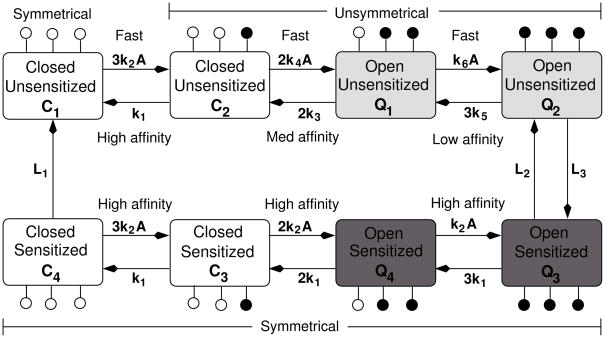
\includegraphics{Yan_P2X7.jpg}

The Yan model is calibrated to BzATP rather than ATP. Since BzATP is reported to be 10 to 50 times more potent an agonist of P2X7 than ATP [sources], but doesn't appear in nature, we had to mathematically convert from ATP to BzATP to make the model more realistic. We opted to do this using a simple multplicative factor on the initial ATP concentration specified.

Each simulation was run with constant value of [ATP], which is unrealistic due to the rapid hydrolization of ATP, unless we assume that ATP is being produced at the same rate that it hydrolyzes.


We ran 1200 (??) second simulations of the Toporikova model with and without the added P2X7 component. Unless otherwise noted, parameter values agreed with those used in Toporikova-Butera [TB Paper].

Although the concentration of IP3 receptors was one of the variables in the Toporikova-Butera paper, we chose to set it to 0.97 (), small enough that it wouldn?t remove voltage dependent frequency from the model, but high enough that calcium still played a role in the bursting pattern. We varied the value of $g_{NaP}$ from 1.8 (below the critical value at 2.0, below which no $I_{NaP}$-induced bursting occurs) to 4.2 nS. The ATP concentration was set at $10^{-6}$ as the highest highest power of [ATP] that didn't cause the bursting pattern to decay to quiescence. Each simulation was run with constant value of [ATP], which is unrealistic due to the rapid hydrolization of ATP, unless we assume that ATP is being expelled into the extracellular medium at the same rate at which it hydrolyzes.


%<Analysis>
Time-series data was analyzed using a Python-based work pipeline developed using the Python module BASS (https://github.com/drcgw/BASS)  (Dobyns et al. submitted) for analyzing waveform data. BASS can be downloaded from https://github.com/drcgw/bass. We extracted interburst interval, burst duration,  intraburst frequency, total cycle time, peaks-per-burst, peak amplitude, and inter-peak interval.<must define these!!!>.

We analyzed the event measures using the data analysis software Prism, developed by GraphPad, with two-way ANOVA tests (p<0.05) to determine statistical significance. 



The Scipy community. (2014) Scipy(Version 0.15.1) [Code Library]. Available at http://scipy.org (Accessed 21 April 2015)

\end{document}

